%xelatex 或 pdflatex 编译
%导言区
\documentclass[UTF8]{article} %UTF8编码
%preface for the main.tex
\usepackage[a4paper]{geometry} %设置纸张为A4大小
\usepackage{hyperref} %可使用超链接(含链接的跳转和一些命令)
\usepackage{amssymb} %提供了额外的数学字体和数学符号
\usepackage{mathtools} %提供了额外的数学工具,如dcases环境
\usepackage{lipsum} %英语假文宏包
\usepackage{graphicx} %插入图片宏包
\usepackage{float} %在浮动体中可使用H选项
\usepackage{extarrows} %提供了额外的箭头,如可随文字延长的各种箭头
\usepackage{array} %可增加更多的表格列限定符
\usepackage{booktabs} %可使用三线表

\usepackage{amsmath} %最常用的数学宏包
\hypersetup{
	colorlinks=true,
	citecolor=magenta,%设置cite类命令超链接的颜色
	linkcolor=blue,%设置目录、脚注、ref等超链接的颜色
	urlcolor=violet,%设置网页超链接的颜色
}

\usepackage[amsmath,thmmarks]{ntheorem} %定理类环境宏包,如果前面使用amsmath宏包,则需加上amsmath宏包选项以避免出现未知问题,若需在定理环境末尾加上特定符号(如证毕符号),则需使用thmmarks宏包选项以使用\theoremsymbol{}命令。
{
	\theoremstyle{plain}
	\setlength{\theoremindent}{0em}
	\newtheorem{definition}{Definition}
}
{
	\theoremstyle{plain}
	\setlength{\theoremindent}{0em}
	\newtheorem{lemma}[definition]{Lemma}
}
{
	\theoremstyle{plain}
	\setlength{\theoremindent}{0em}
	\newtheorem{theorem}[definition]{Theorem}
}
{
	\theoremstyle{plain}
	\setlength{\theoremindent}{0em}
	\newtheorem{corollary}[definition]{Corollary}
}
{
	\theoremstyle{nonumberplain}
	\setlength{\theoremindent}{0em}
	\theorembodyfont{\normalfont}
	\theoremsymbol{$\blacksquare$} %在证明环境末尾加上一个证毕符号
	\newtheorem{proof}{Proof}
}

%定义新命令与新运算符
\DeclareMathOperator{\diff}{d\!}
\newcommand{\var}{\mathrm{Var}}
\newcommand{\cov}{\mathrm{Cov}}

%标题页设置
\title{
	A homework template
}
\author{Meiting Wang\thanks{Meiting Wang, Email: wangmeiting92@gmail.com}}
\date{\today}




%正文区
\begin{document}
\maketitle

\begin{enumerate}
    \item \lipsum[1][1-3] %problem boundary--------------------------------------------------------------------
    \begin{enumerate}
        \item \lipsum[2][2-3]
        
        The solution for this section will be as follows ...
        
        \item \lipsum[2][2-3]
        
        \begin{lemma}
            \lipsum[3][2-3]
            \[ a^2 + b^2 = c^2 \]
            The equation above depict a fact that ...
        \end{lemma}
        
        \begin{lemma}[xxx]\label{lemma:xxx}
            \lipsum[3][2-3]
        \end{lemma}
        
        As the Lemma \ref{lemma:xxx} said, ...
        
        \item \lipsum[2][2-3]
        
        \begin{theorem}
            \lipsum[1][1-4]
        \end{theorem}
        
        \begin{proof}
            \lipsum[3][1-3]
        \end{proof}
        
    \end{enumerate}
    \item \lipsum[1][1-3] %problem boundary--------------------------------------------------------------------
    \begin{enumerate}
        \item \lipsum[2][2-3]
        
        \lipsum[1][1-8]
        
        \item \lipsum[2][2-3]
        
        \begin{table}[H]
        	\centering
        	\caption{Descriptive statistics}\label{tab:stat}
        	\begin{tabular}{l*{5}{>{$}c<{$}}}
        		\toprule
        		&\text{count}&\text{mean}&\text{sd}&\text{min}&\text{max}\\
        		\midrule
        		price       &          74&    6165.25&    2949.49&        3291&       15906\\
        		mpg         &          74&     21.29&    5.78&          12&          41\\
        		weight      &          74&    3019.45&    777.19&        1760&        4840\\
        		rep78       &          69&    3.4057&    .98&           1&           5\\
        		\bottomrule
        	\end{tabular}
        \end{table}
        
        As table \ref{tab:stat} shows, ...
        
        \begin{figure}[htbp]
        	\centering
        	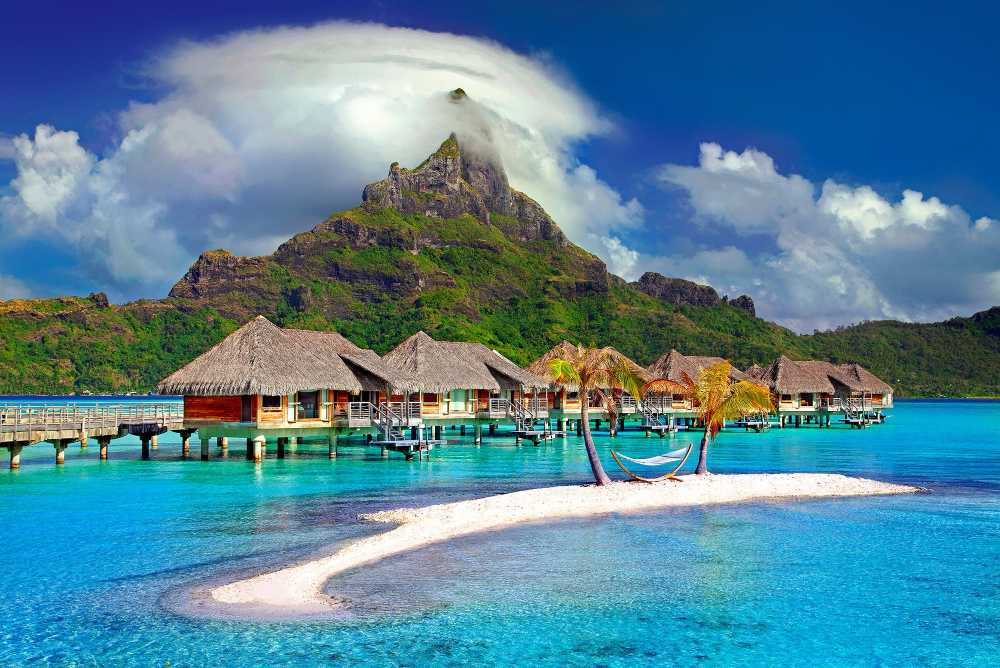
\includegraphics[width=0.5\textwidth]{1.jpg}
        	\caption{Beautiful scenery} \label{fig:scenery}
        \end{figure}
        
        As the figure \ref{fig:scenery} shows, ...
        
        \item \lipsum[2][2-3]
        
        \begin{gather}
            a + b = c \\
            a + b = c \label{eq:abc} \\
            a + b = c 
        \end{gather}
        
        As the equation \eqref{eq:abc} shows, ...
    \end{enumerate}
\end{enumerate}





\end{document}
